\documentclass{beamer}
\usepackage[ngerman]{babel}
\usepackage[utf8]{inputenc}     % UTF8-Encoding
\usepackage[T1]{fontenc}        % T1-Schriftkodierung
\usepackage{lmodern}            % Ersetzung der CM-Schrift
\usepackage{listingsutf8}       % Listings (mit UTF8)
\usepackage{array}              % neue Spaltenmodi
\usepackage{textcomp}           % spezielle Zeichen im Text
\usepackage[ngerman]{varioref}  % variable Verweise
\usepackage{scrextend}          % für Labeling
\usepackage{booktabs}           % spezielle Linien in Tabellen
\usepackage{graphicx}

\makeatletter

% Anpassung des CambridgeUS Beamerthemes mit Ubuntufarben von Eremit7. This work is under the GPL v2.
% This is Version 1.1 (12. Okt. 2011)
% This file is made for Xelatex. To compile the packages “texlive-xetex” and „ttf-ubuntu-font-family” must be installed. Then run “xelatex vorlage.tex“ (note the xeLAtex).
% Make sure that circle_of_friends.pdf is found and beamerouterthemeubuntulines.sty is in the texmf path or the same directory as the .tex file.

% Packages for Xelatex
\usepackage{fontspec}
\usepackage{xltxtra}
\usepackage{polyglossia}% babel for Xelatex
\setdefaultlanguage{english}% Set the Language for ployglossia

% Define the Orange from the Ubuntu branding.
\definecolor{Ubuntu-Orange}{RGB}{221,072,20}

% Load the Theme.
\usetheme{CambridgeUS}

% I never saw anybody using the navigation symbols, so disable them.
\setbeamertemplate{navigation symbols}{}

% Substitute the red in the Theme with the predefined Ubuntu-Orange.
\setbeamercolor{palette primary}{fg=Ubuntu-Orange}
\setbeamercolor{palette secondary}{fg=Ubuntu-Orange}
\setbeamercolor{palette tertiary}{bg=Ubuntu-Orange}
\setbeamercolor{titlelike}{fg=Ubuntu-Orange}
\setbeamercolor{item}{fg=Ubuntu-Orange}
\setbeamercolor{block title}{fg=Ubuntu-Orange}

% Now commes the Ubuntu font.
% Because of beamers shortcomings we need to use a workaround: 
% This beamer fonttheme uses sansserif for the normal text and 
% serif fonts for the rest
\usefonttheme[stillsansseriftext]{serif}

% Now we tell XeLaTex what fonts to use: For the sansserif font Ubuntu Light and as the “serif” font Ubuntu. Ubuntu isn't an serif font, but this way XeLaTex sets all text that was defined as “serif“ in the line above in the Ubuntu font.
 % Using only the Ubuntu font would result in to heavy text.
\defaultfontfeatures{Ligatures=TeX,Scale=MatchLowercase} % Set the features for every font, the first enables the usual TeX Ligatures (e. g. --- = —) and the second scales the fonts to the same height
\setsansfont{Ubuntu Light}
\setmainfont{Ubuntu}
\setmonofont{DejaVu Sans Mono} % Use this when using a pre-oneiric ubuntu-font-package (Monospaced fonts were added in Oneiric)
%\setmonofont{Ubuntu Mono}% Works only with lualatex duo to bug: 867853 (in Launchpad)

\titlegraphic{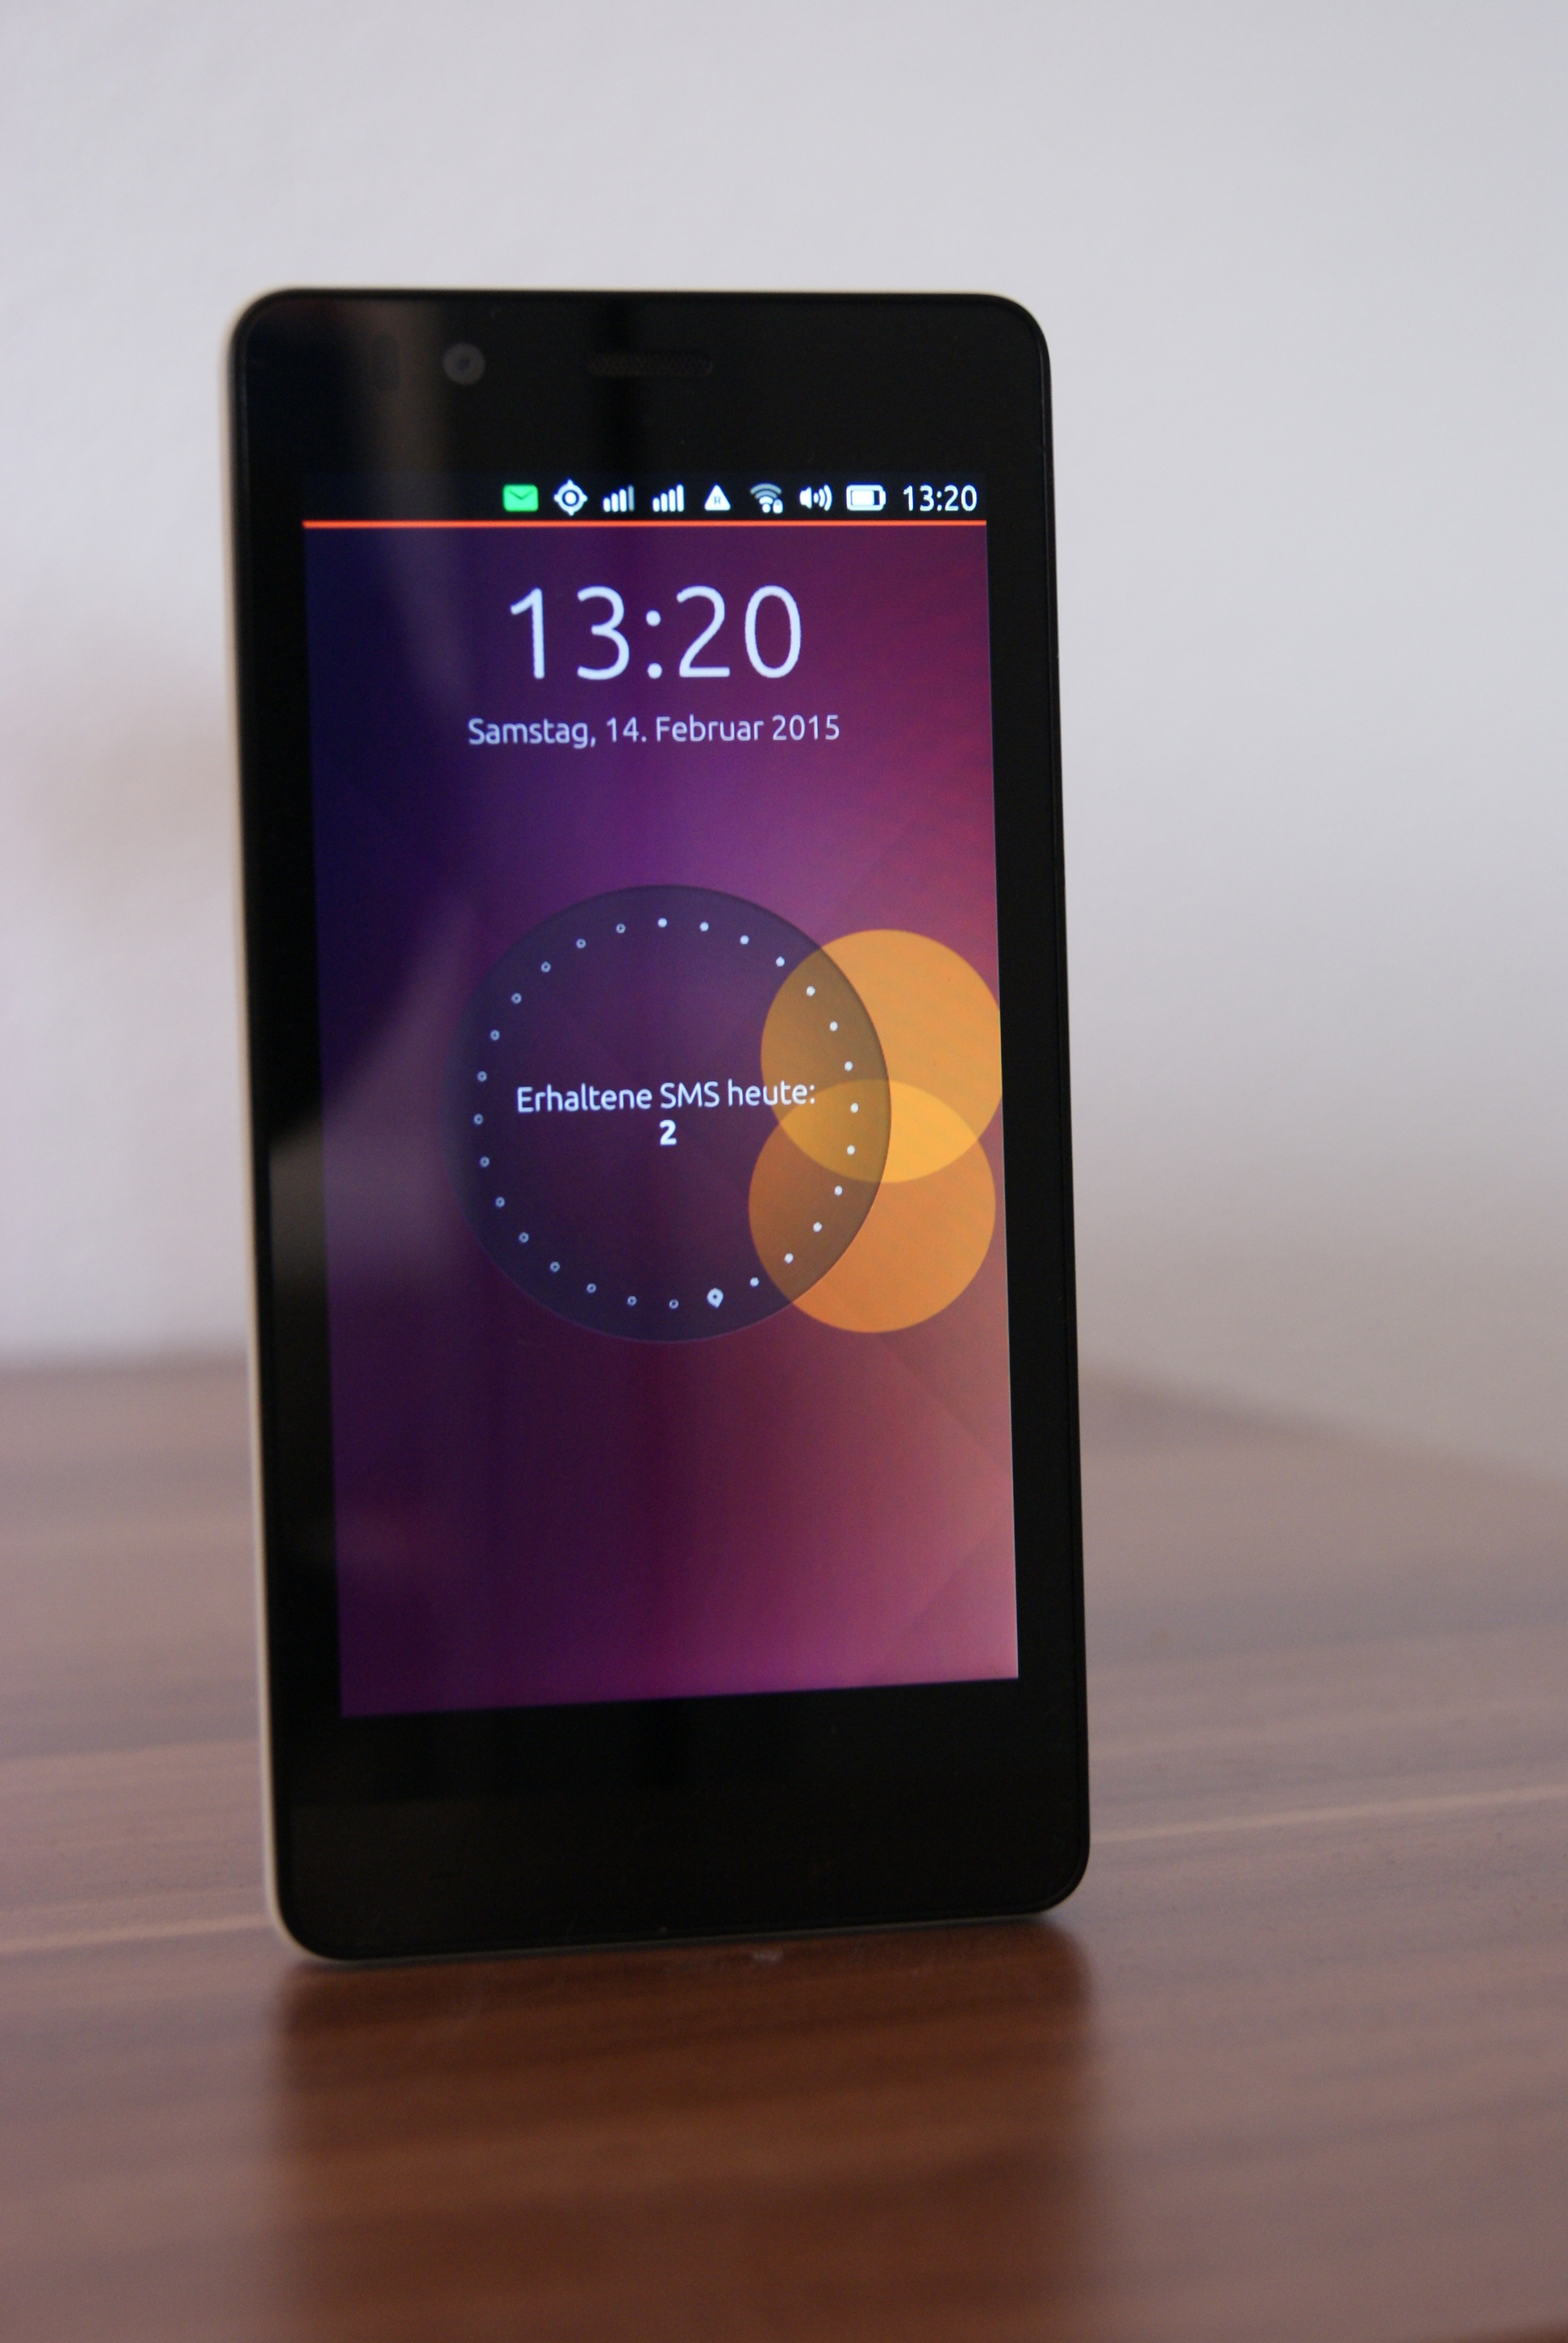
\includegraphics[width=0.2\linewidth]{images/ubuntuphone}}
\title{Ubuntu Phone}
\author[Sujeevan Vijayakumaran]{Sujeevan Vijayakumaran\\

\includegraphics[width=0.3\linewidth]{images/name.png}\\
\tiny{oder auch: Er, dessen Name nicht genannt wird.}}
\date{22. August 2015}
\institute{FrOSCon}

\begin{document}
\maketitle
\begin{frame}
  \frametitle{Inhaltsverzeichnis}
  \tableofcontents
\end{frame}

\section{Bedienung und Konzepte}

\frame{\sectionpage}

\begin{frame}
  \frametitle{Bedienkonzepte}
  \begin{columns}
    \column[c]{.33\textwidth}
      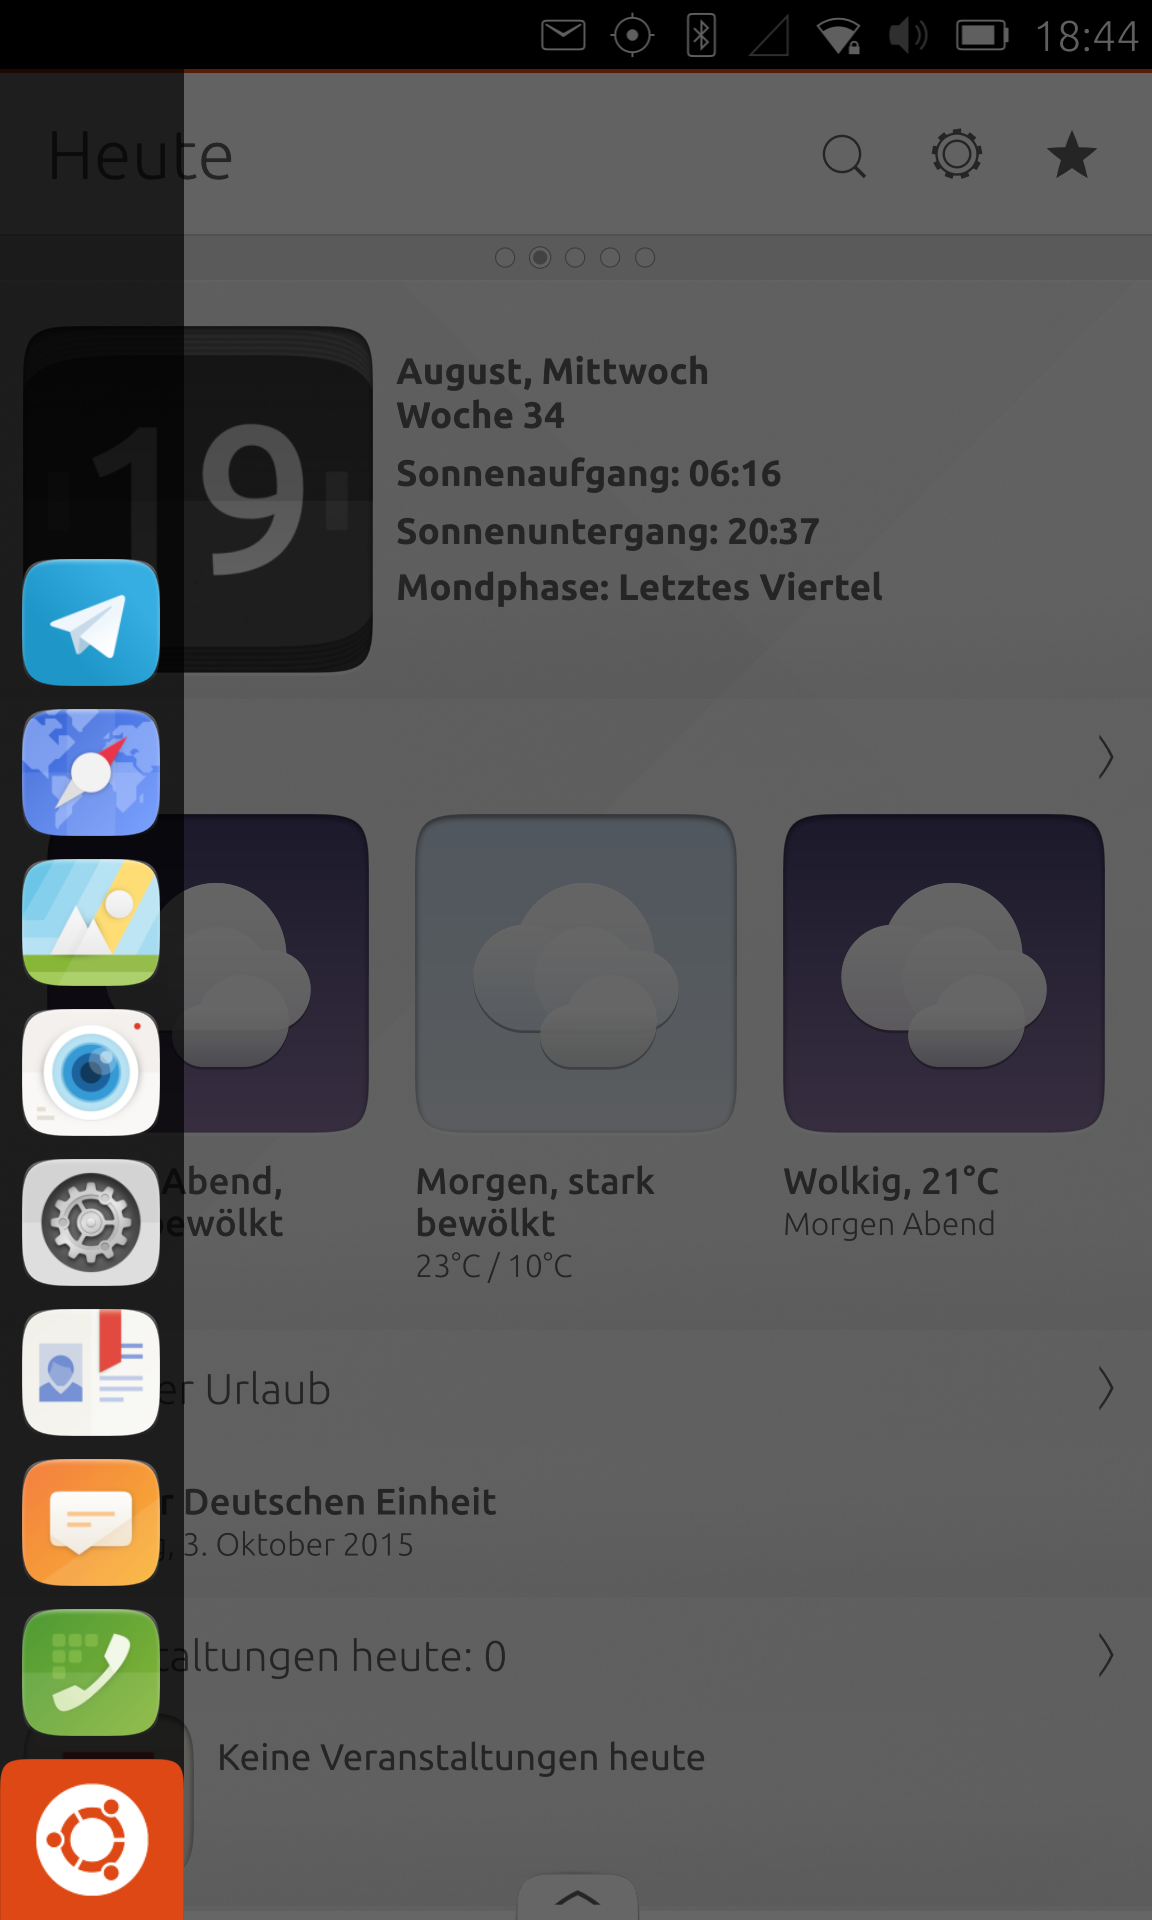
\includegraphics[width=\textwidth]{images/unity-launcher}
    \column[c]{.33\textwidth}
      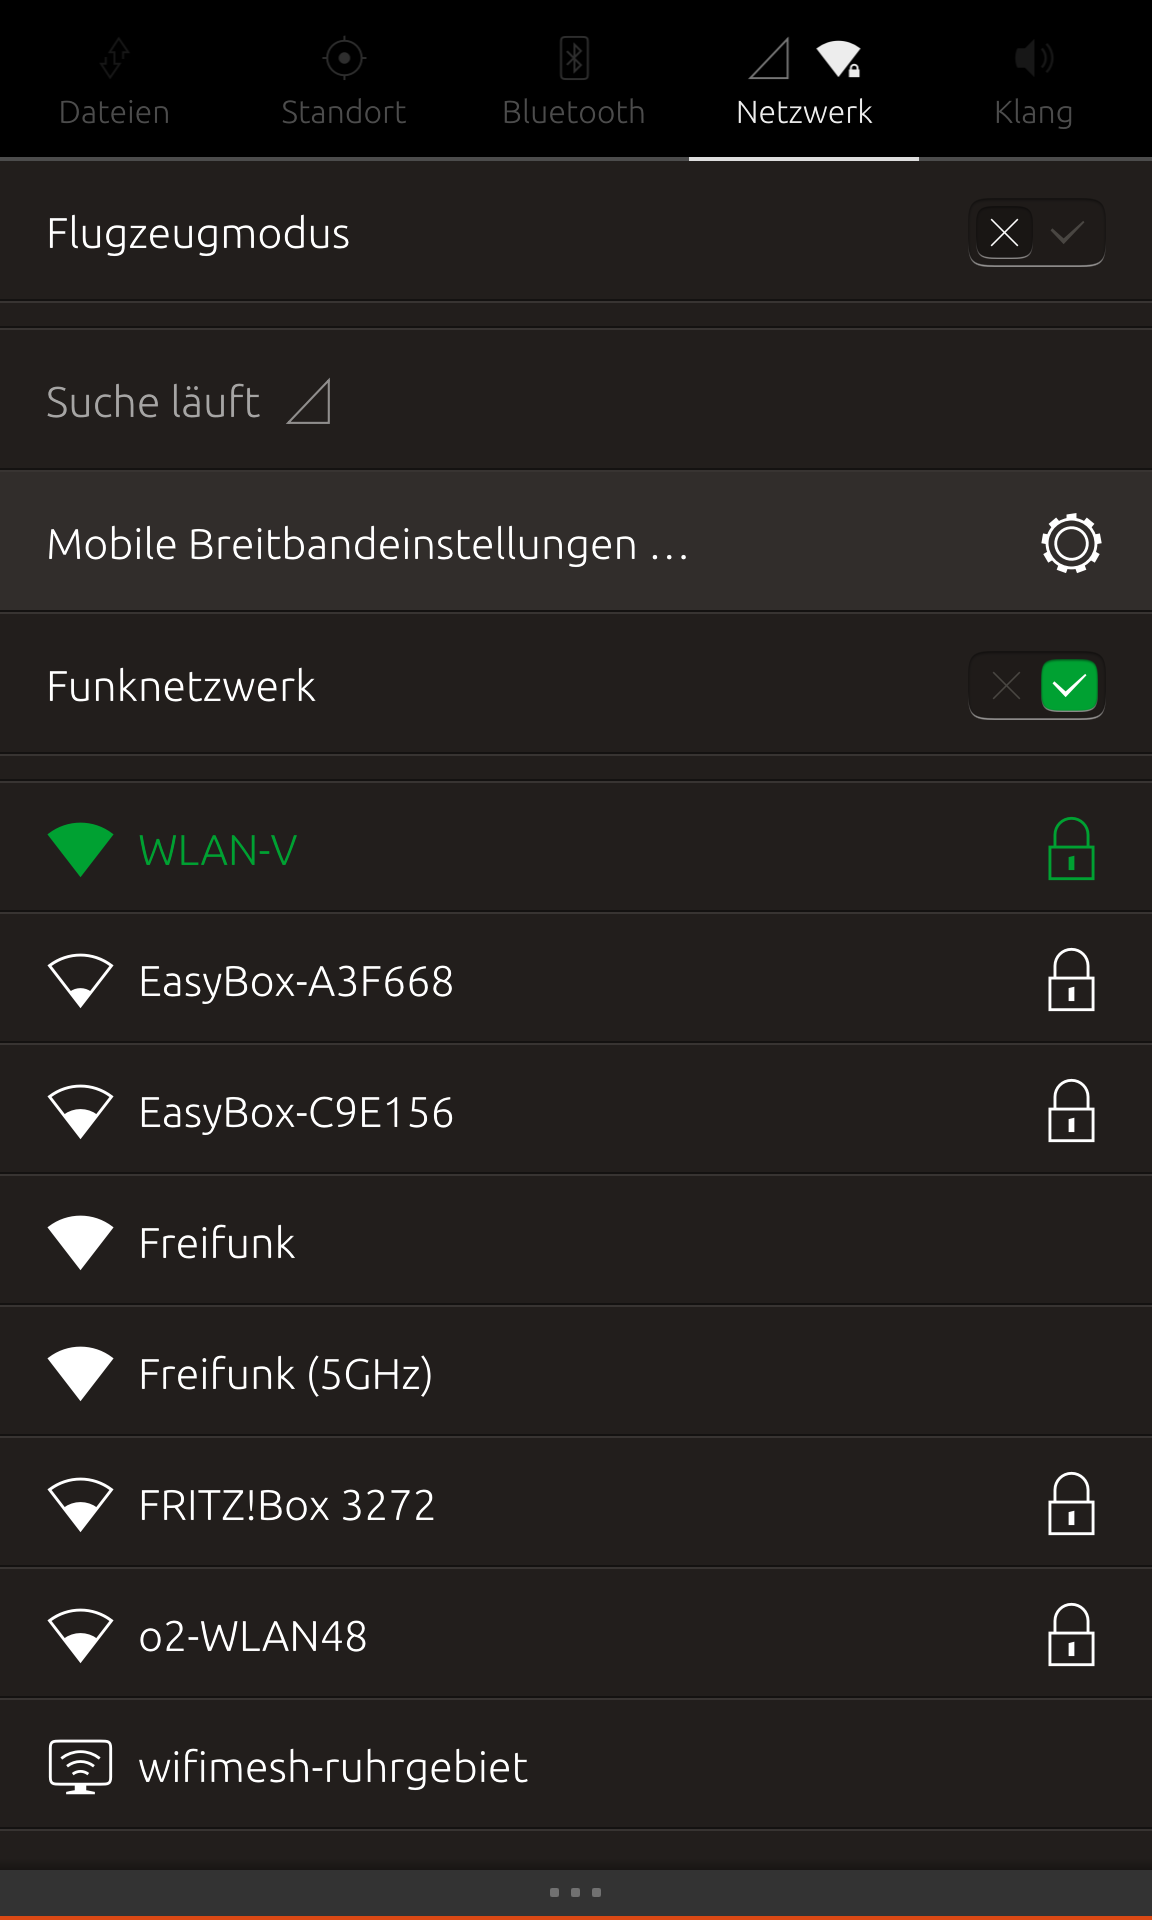
\includegraphics[width=\textwidth]{images/wlan}
    \column[c]{.33\textwidth}
      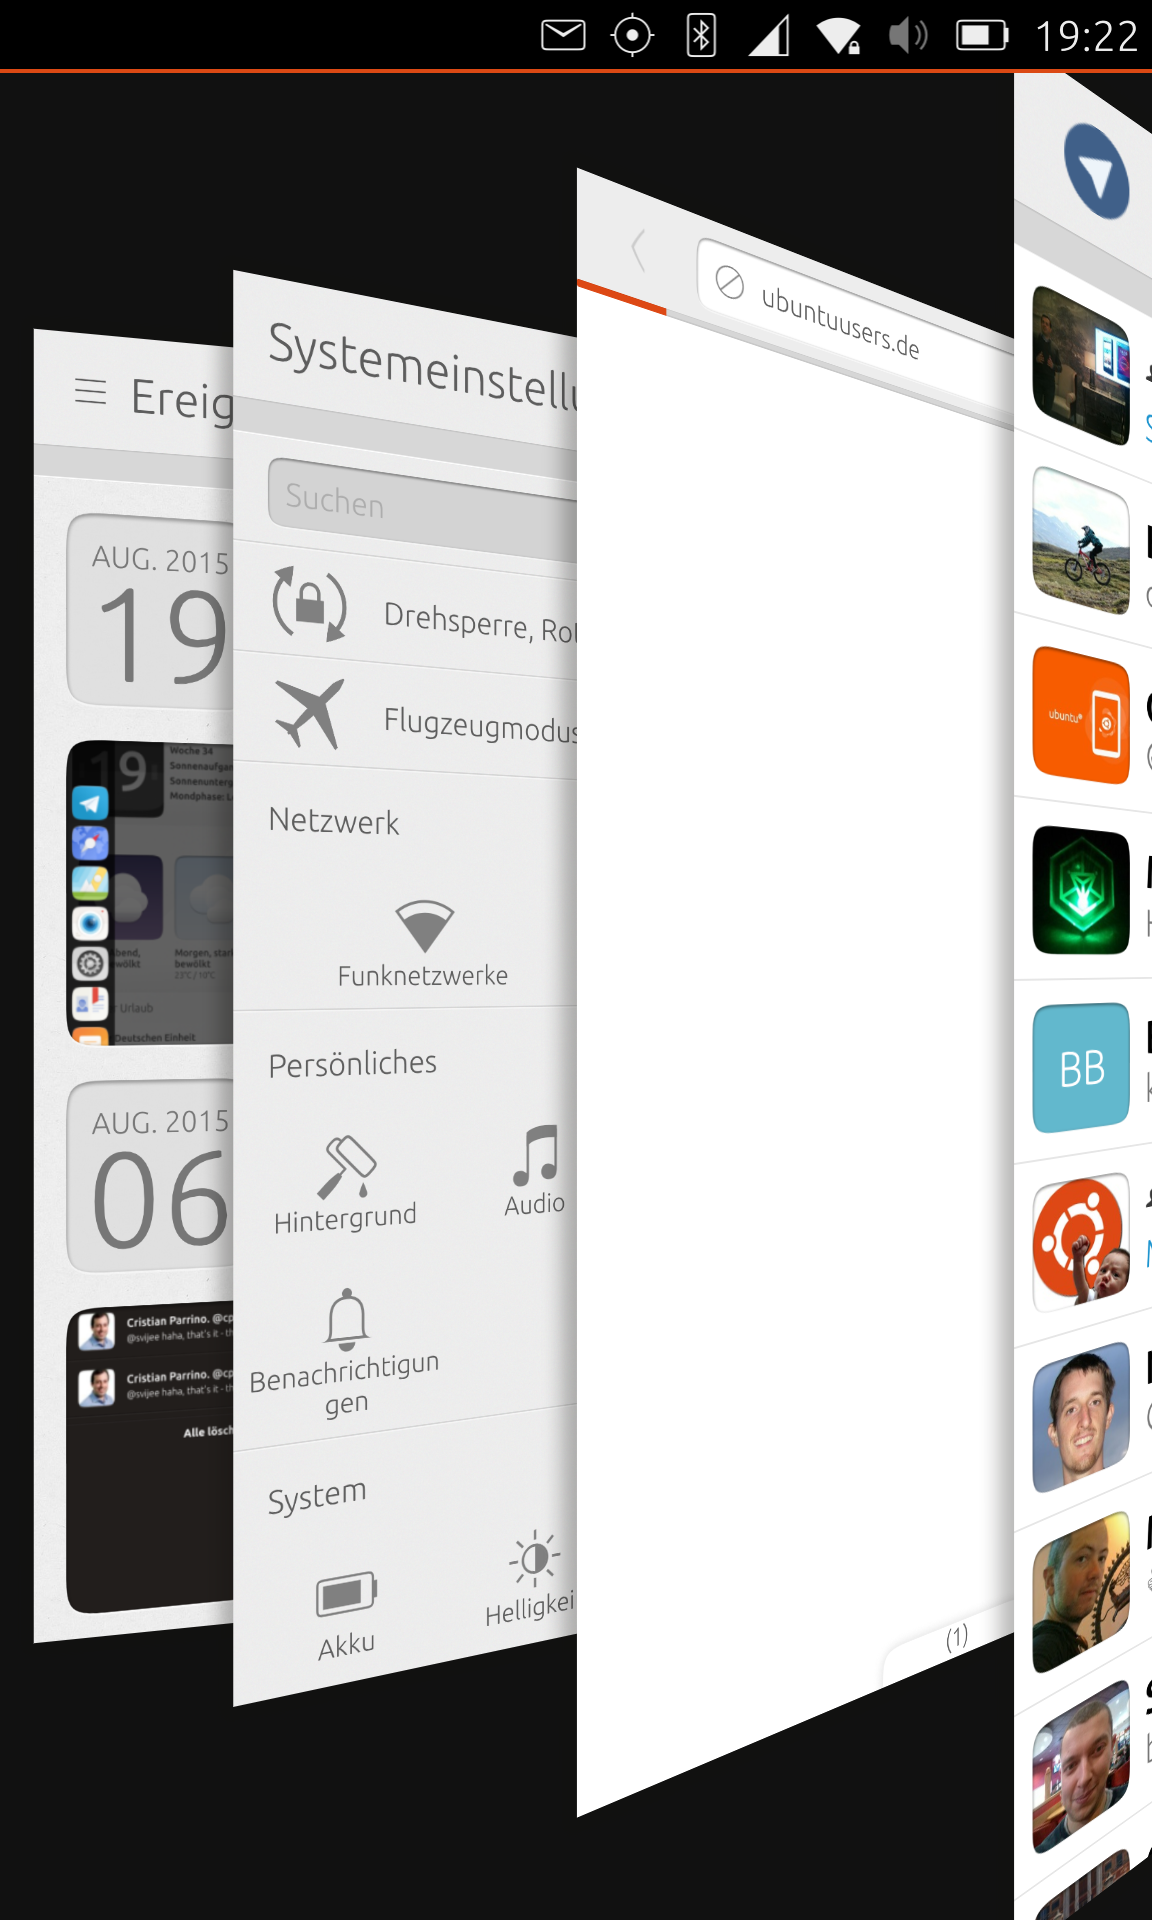
\includegraphics[width=\textwidth]{images/appswitcher}
  \end{columns}
  
\end{frame}

\begin{frame}
  \frametitle{Scopes}
  \begin{columns}
    \column[c]{.50\textwidth}
      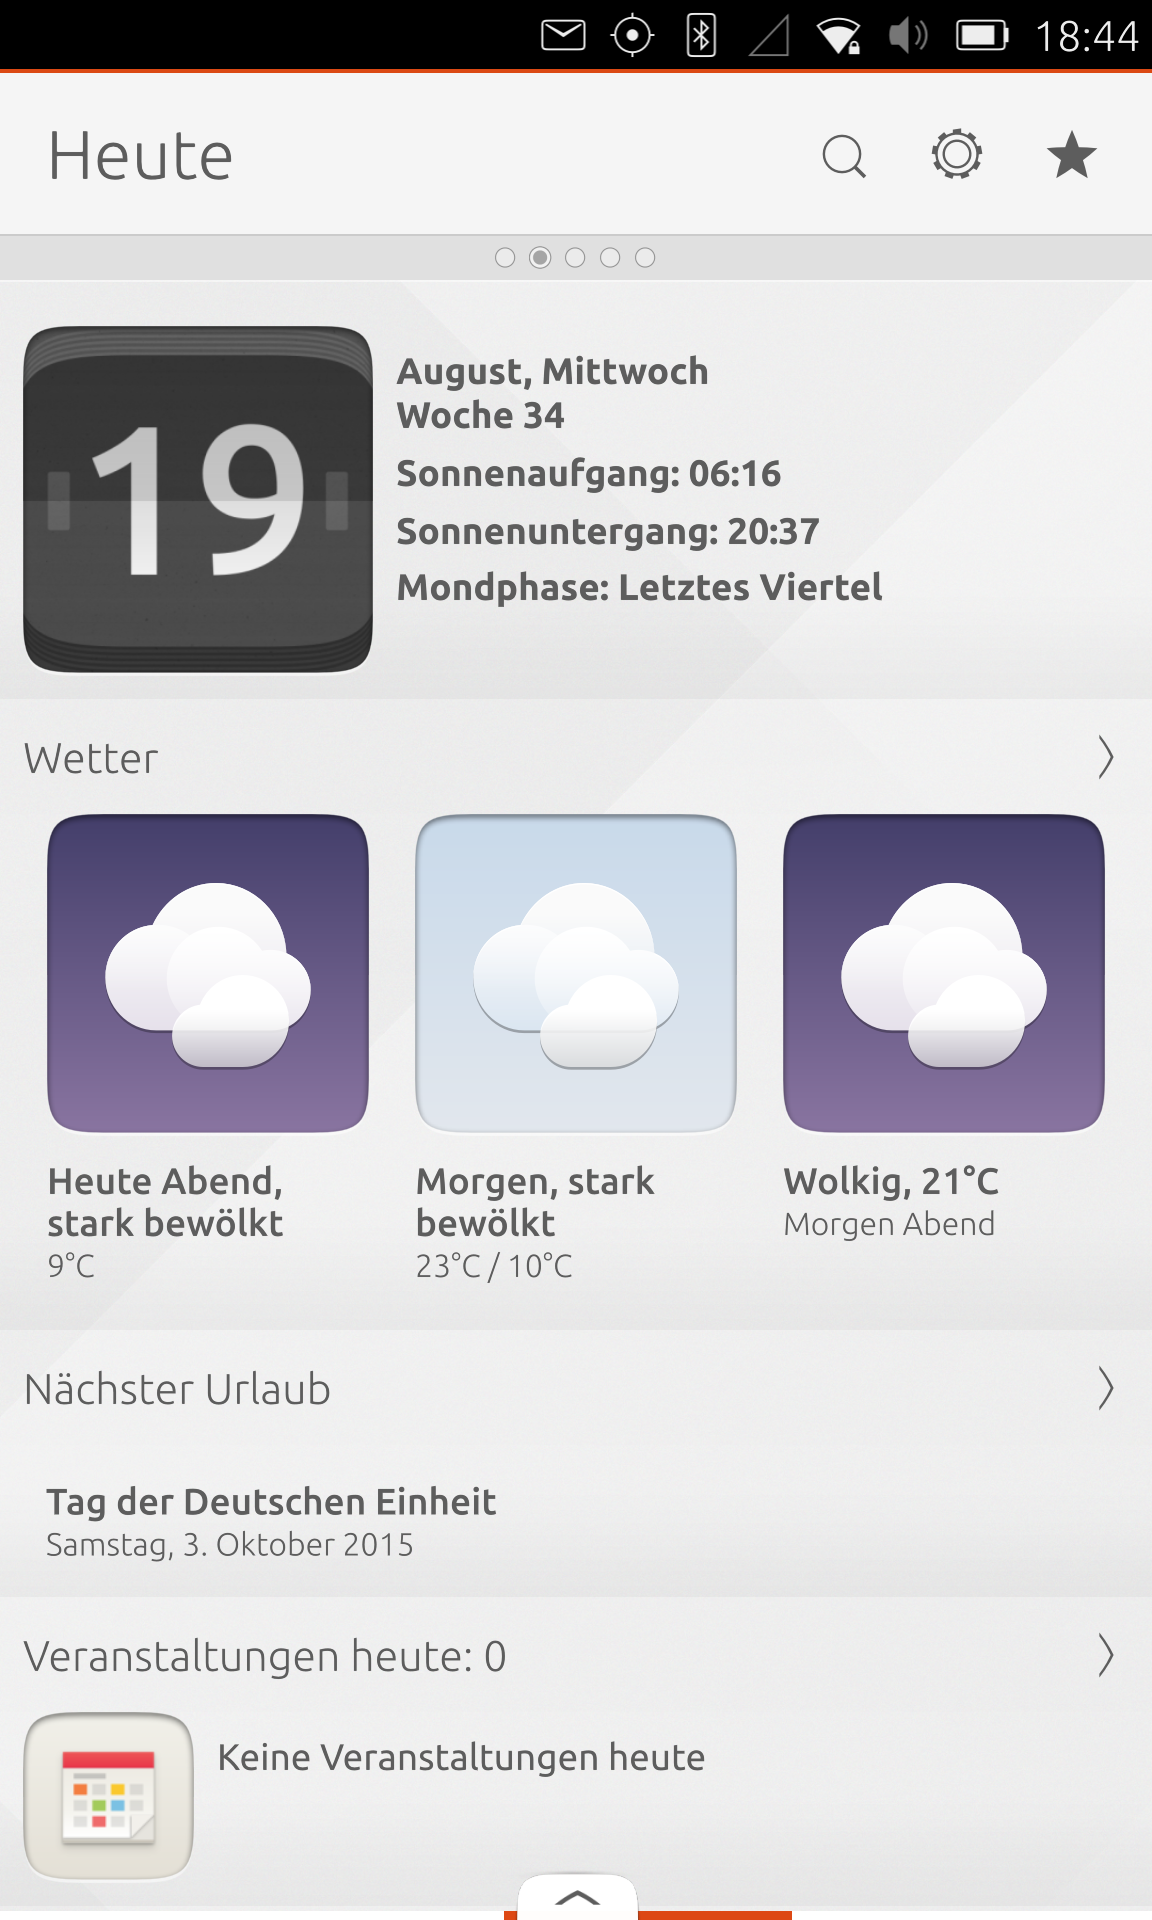
\includegraphics[width=0.7\textwidth]{images/scope}
    \column[c]{.50\textwidth}
      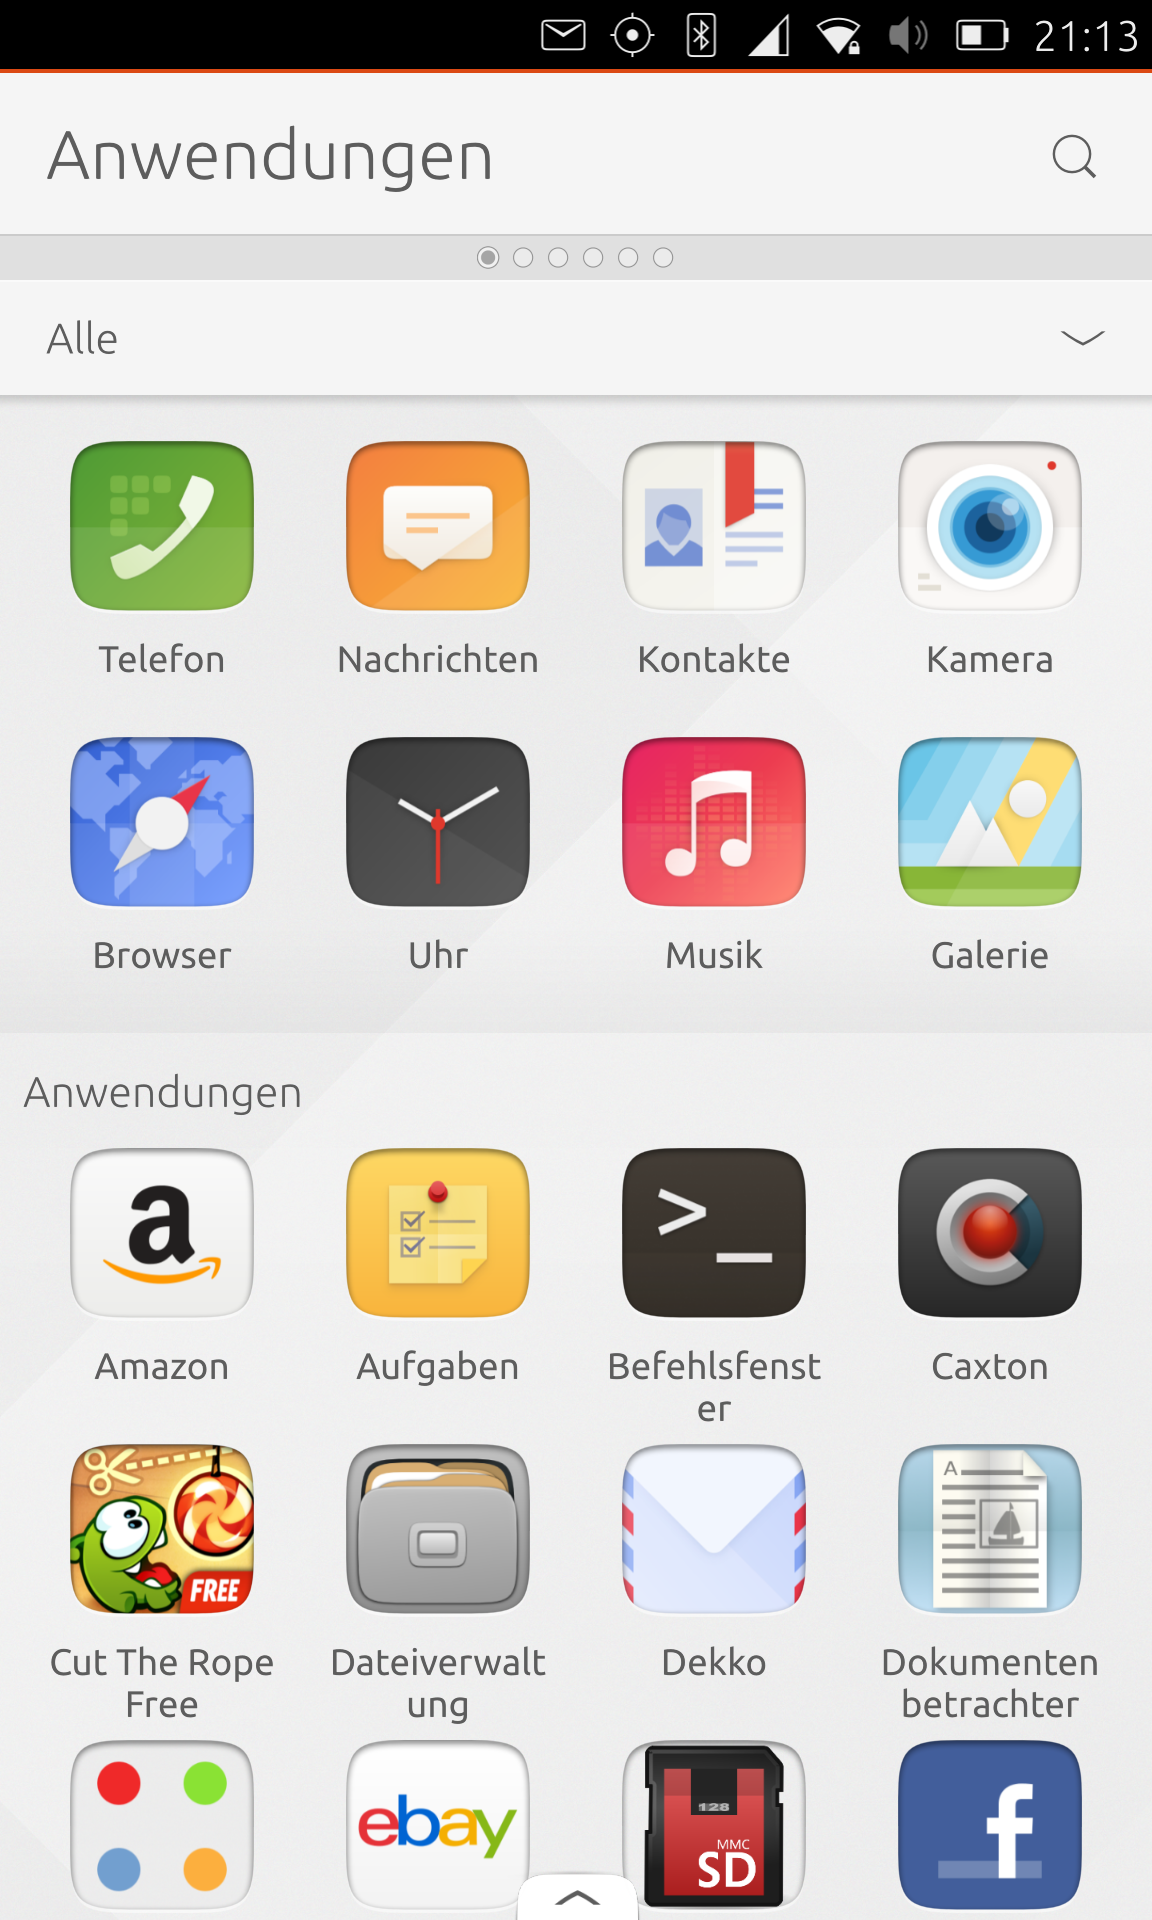
\includegraphics[width=0.7\textwidth]{images/applauncher}
  \end{columns}
\end{frame}

\section{Geräte und Märkte}

\frame{\sectionpage}

\begin{frame}
  \frametitle{bq Aquaris E4.5}
  \begin{columns}
    \column[c]{.50\textwidth}
      \begin{itemize}
        \item 4,5" mit 540 x 960
        \item MediaTek Quad Core Cortex A7 bis 1,3 GHz
        \item 8GB interner Speicher + micro SD Slot (max 32GB)
        \item 1GB RAM
        \item 2x micro-SIM
        \item Preis: 170€
      \end{itemize}
    \column[c]{.50\textwidth}
      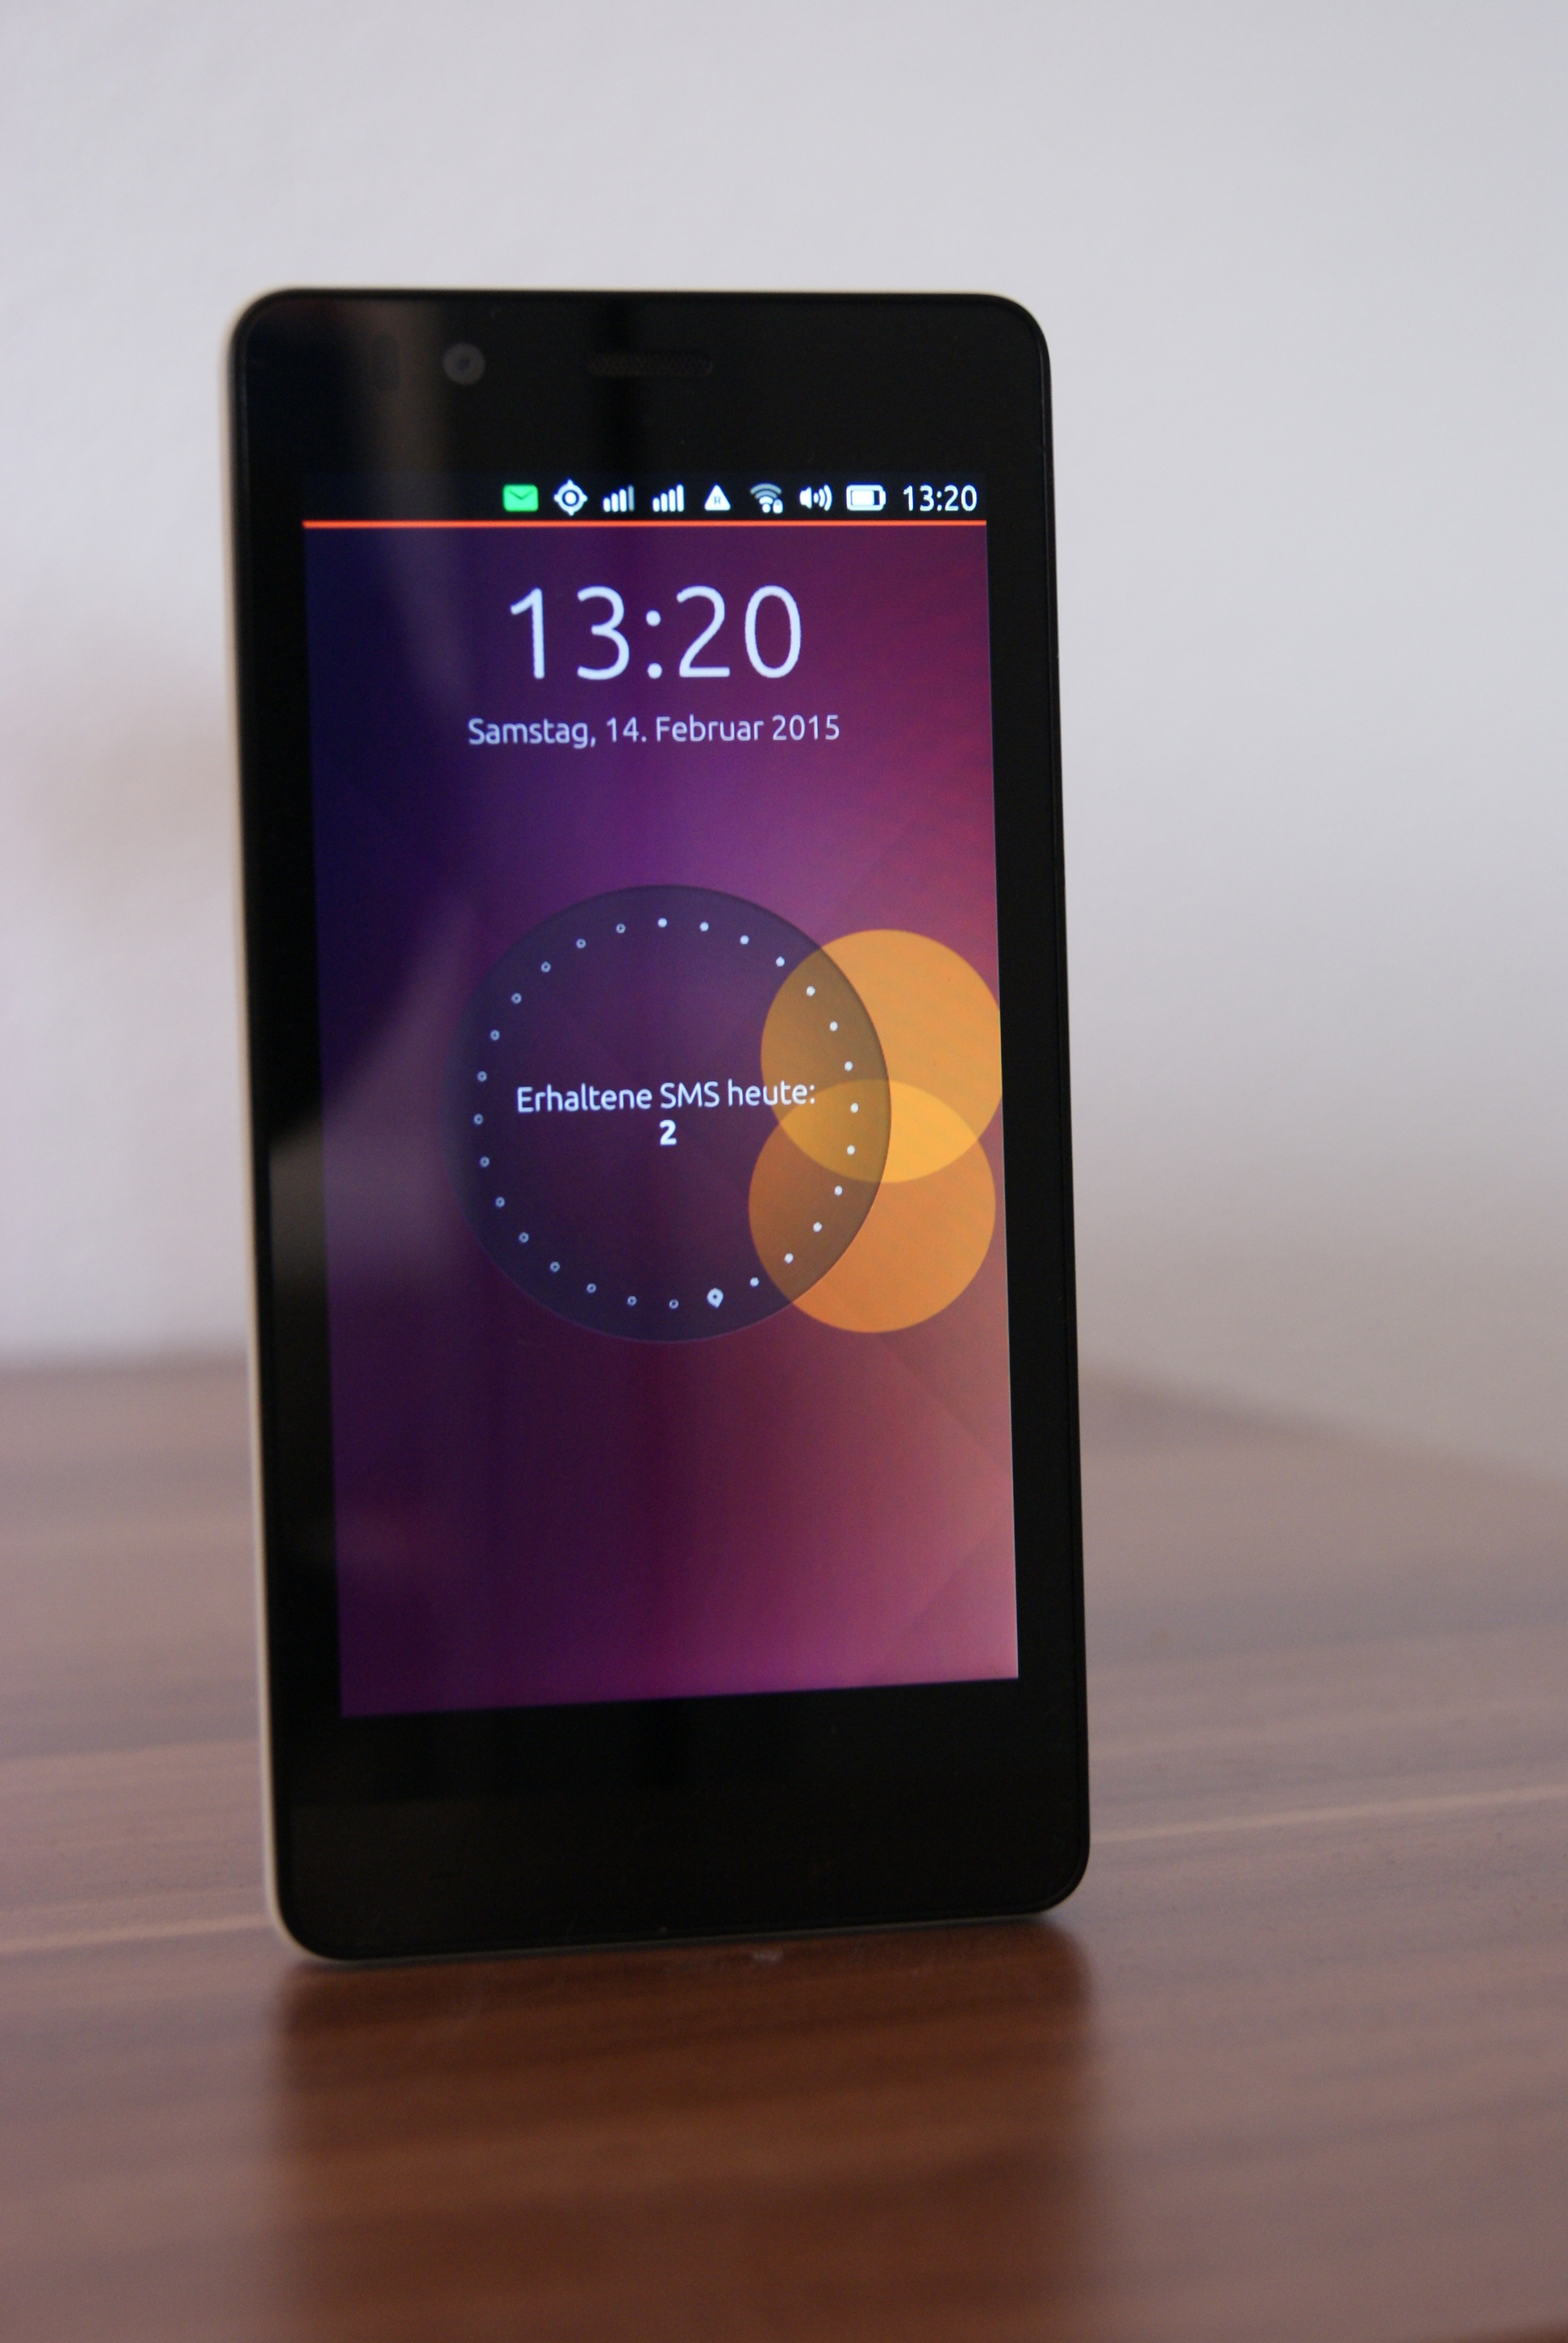
\includegraphics[width=0.8\textwidth]{images/ubuntuphone}
  \end{columns}
\end{frame}

\begin{frame}
  \frametitle{bq Aquaris E5}
  \begin{columns}
    \column[c]{.50\textwidth}
      \begin{itemize}
        \item 5" mit 720 x 1280
        \item MediaTek Quad Core Cortex A7 bis 1,3 GHz
        \item 16GB interner Speicher + micro SD Slot (max 32GB)
        \item 1GB RAM
        \item 2x micro-SIM
        \item Preis: 200€
      \end{itemize}
    \column[c]{.50\textwidth}
      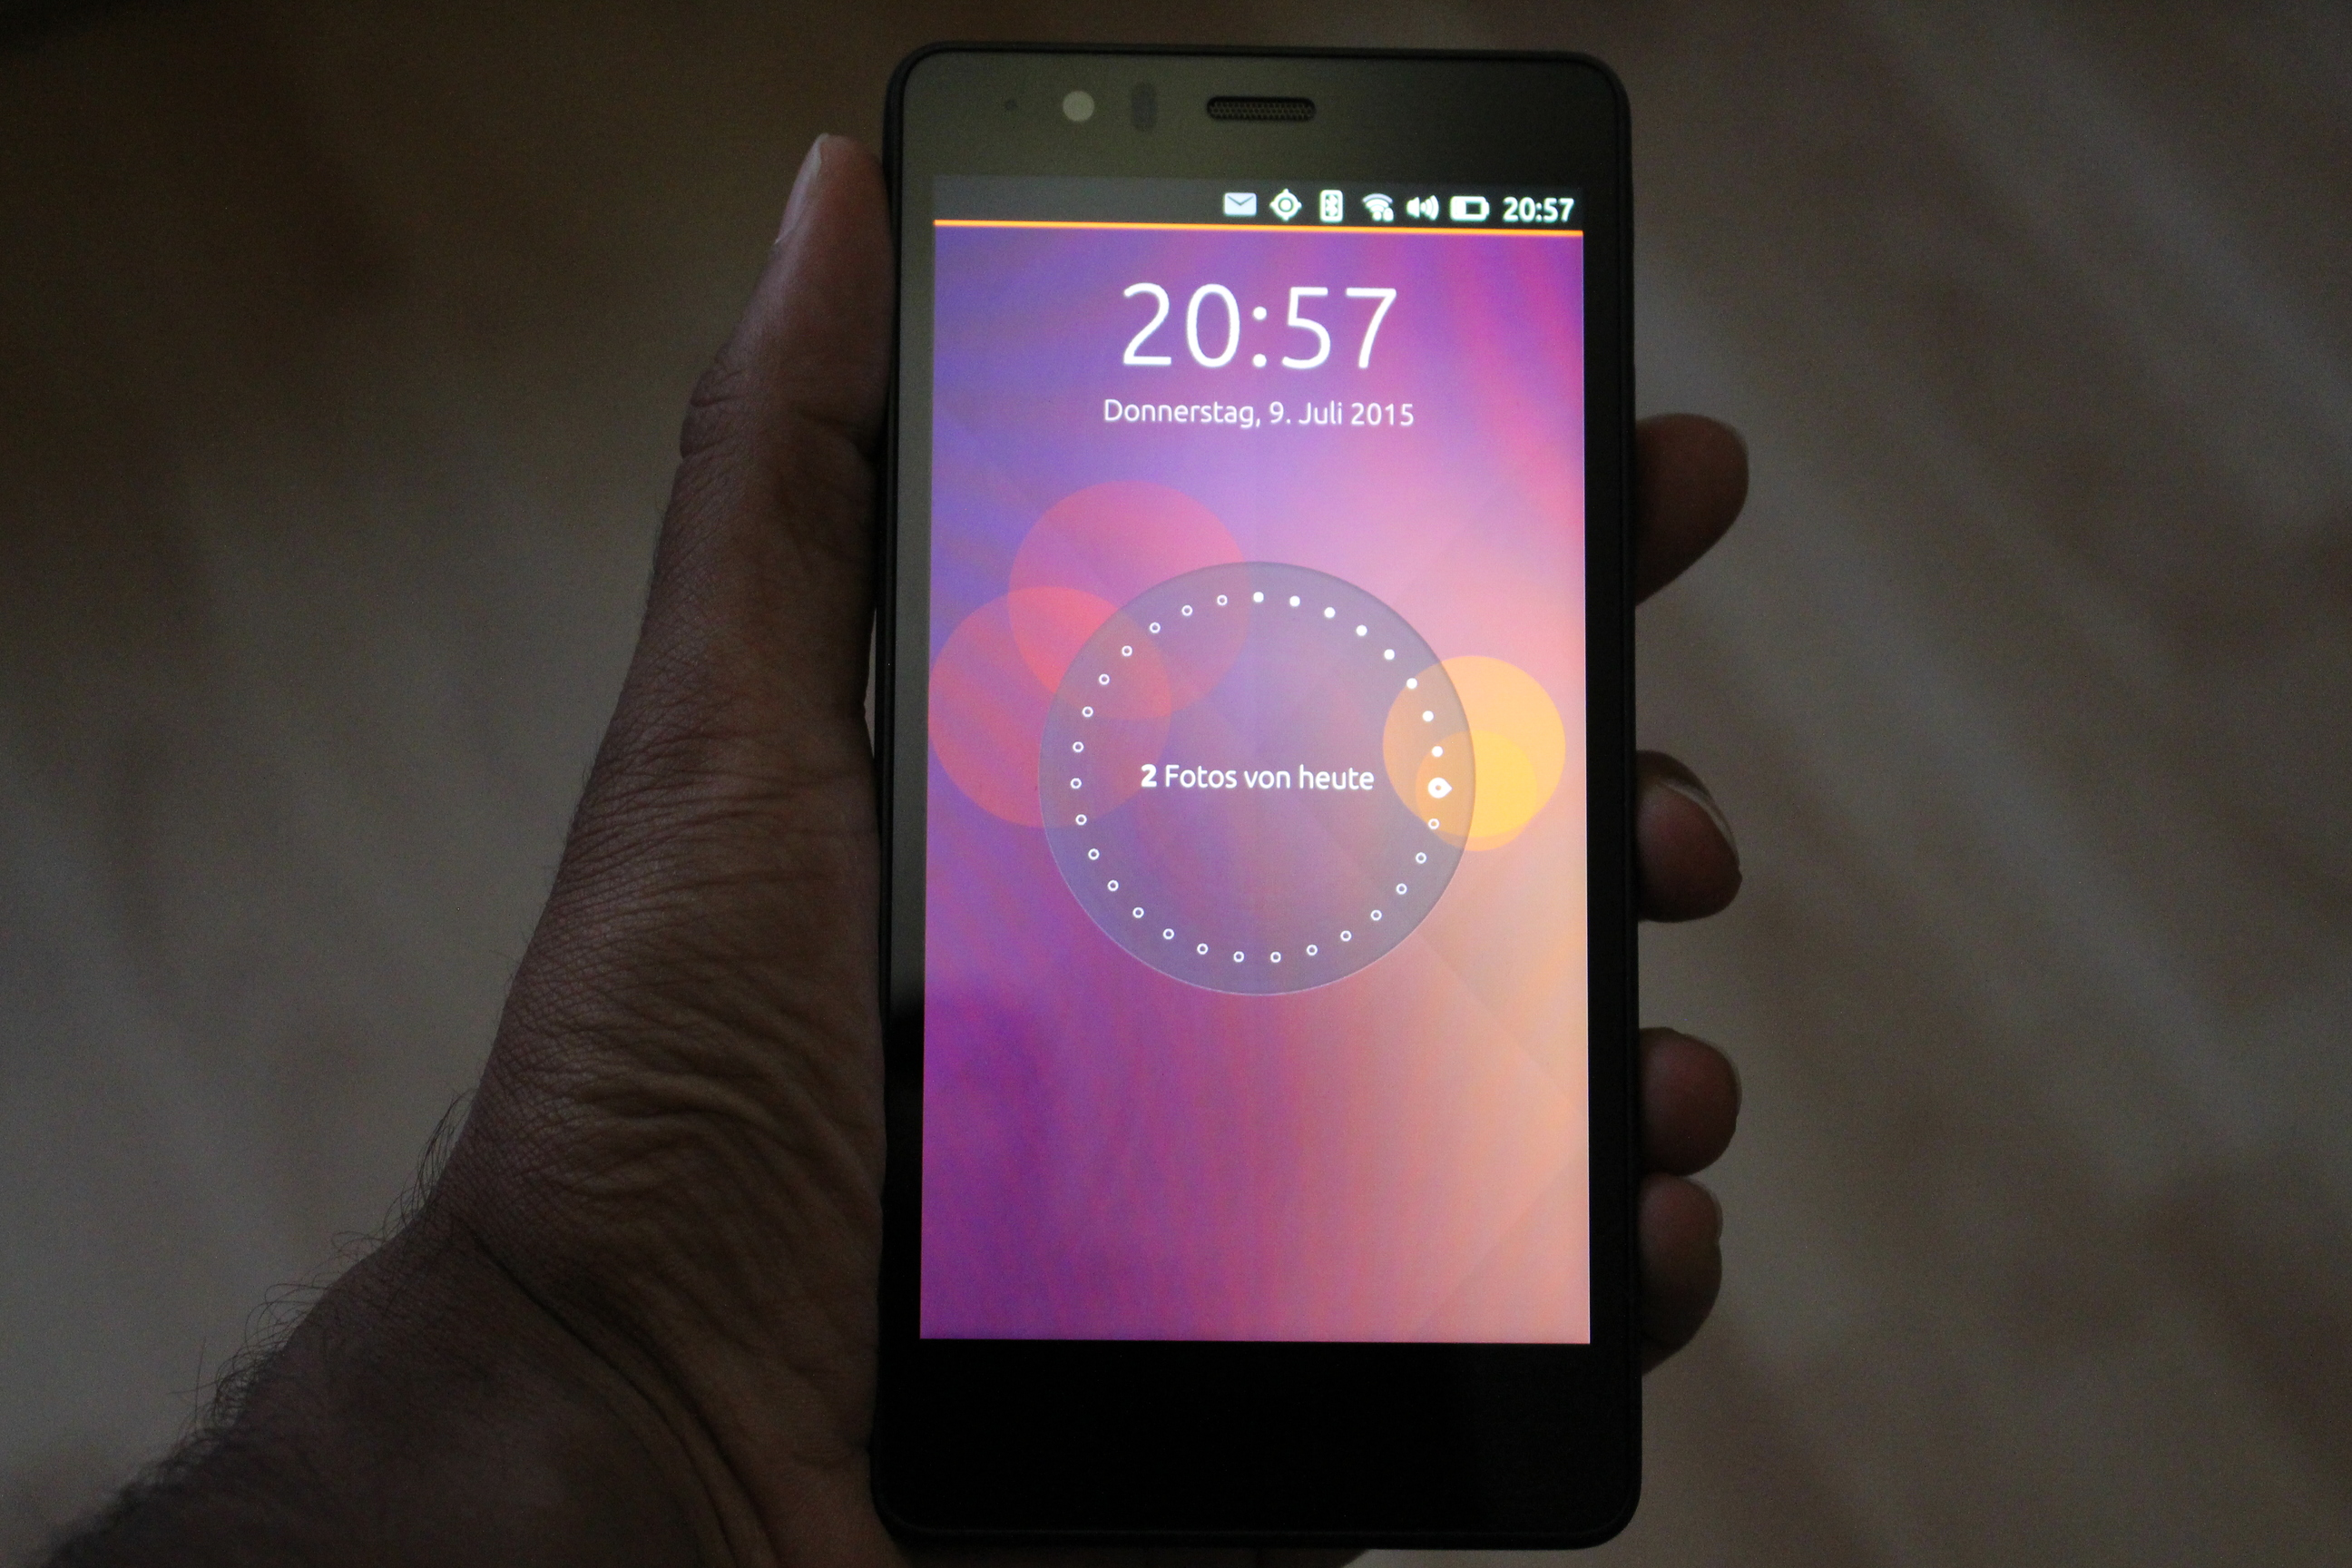
\includegraphics[width=0.8\textwidth]{images/e5}
  \end{columns}
\end{frame}

\begin{frame}
  \frametitle{Meizu MX4}
  \begin{columns}
    \column[c]{.50\textwidth}
      \begin{itemize}
        \item 5,4" mit 1920 x 1152
        \item MediaTek Octa-Core (Big.LITTLE-Architektur)
        \item 16GB interne Speicher (keine micro SD!)
        \item 2GB RAM
        \item 20,7 Megapixel Kamera
        \item Preis: 300€
      \end{itemize}
    \column[c]{.50\textwidth}
      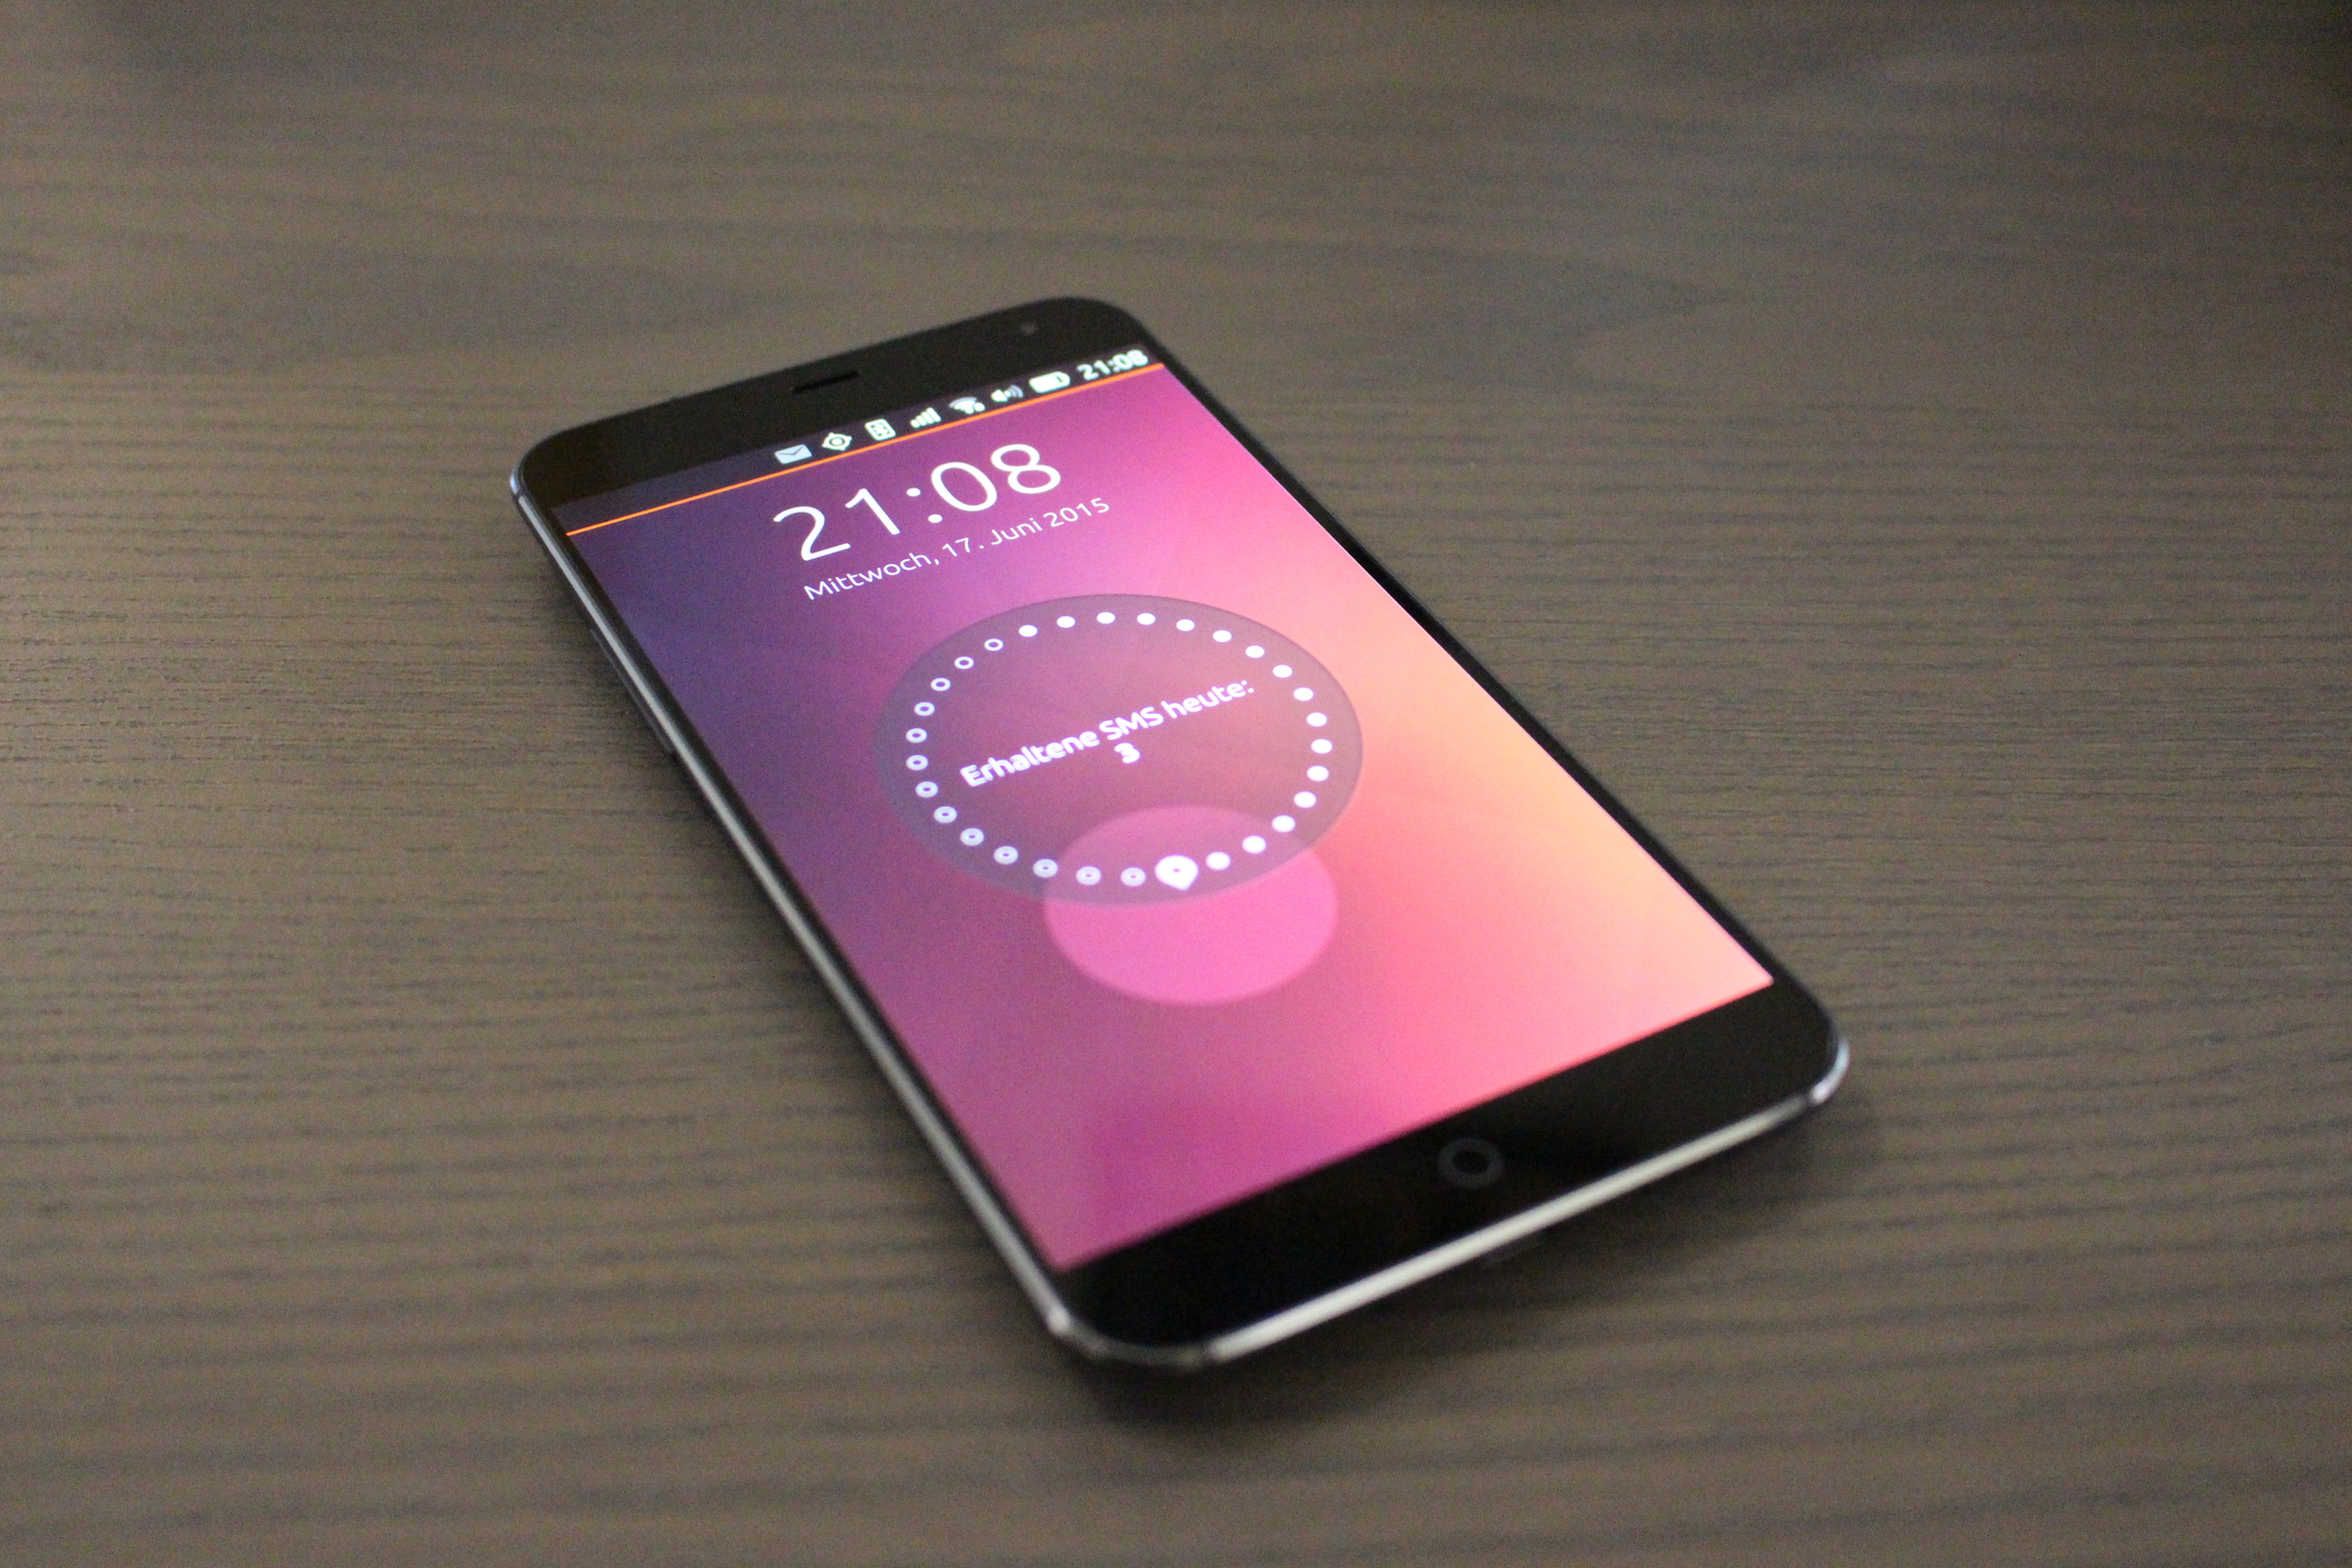
\includegraphics[width=0.8\textwidth]{images/meizumx4}
  \end{columns}
\end{frame}

\section{System-Aufbau}

\frame{\sectionpage}

\begin{frame}
  \frametitle{System-Architektur}
  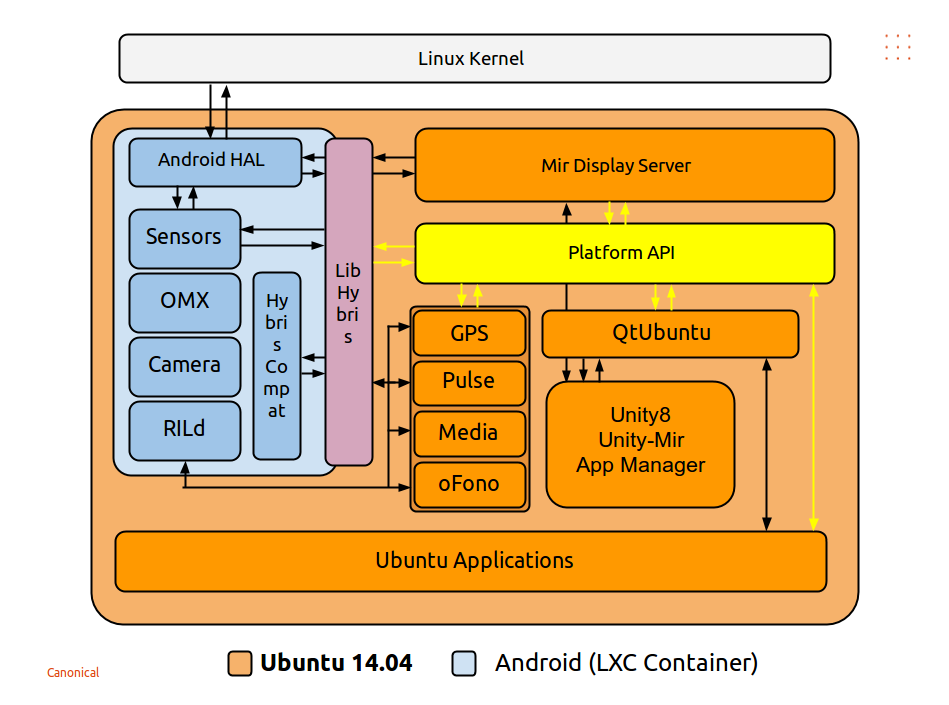
\includegraphics[width=0.9\textwidth]{images/ubuntu_touch_architecture}
\end{frame}

\begin{frame}
  \frametitle{System-Architektur}
  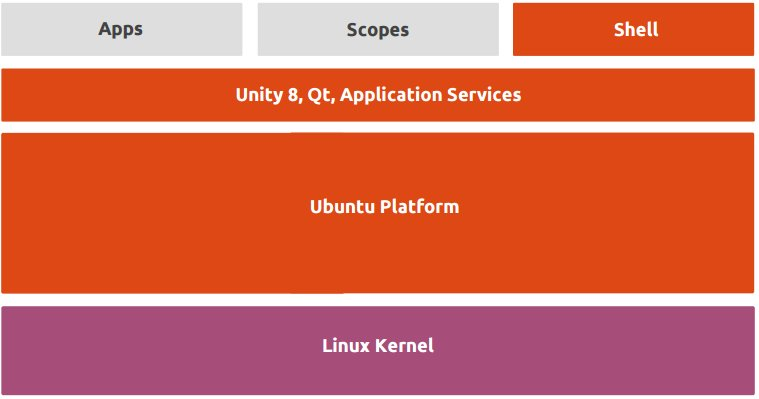
\includegraphics[width=0.9\textwidth]{images/system-arch2}
\end{frame}

\begin{frame}
  \frametitle{Was ist drin?}
  \begin{itemize}
    \item (fast) der selbe Kernel
    \item die selben Platform Services*
    \item die selben GNU Tools
    \item das selbe Paket-Archiv
    \item die selbe Unity-Shell*
  \end{itemize}

  * zur Zeit noch nicht das selbe auf Desktop und Phone
\end{frame}

\begin{frame}
  \frametitle{Neue Technologien}
  \begin{itemize}
    \item Mir
    \item Click packages (statt deb)
    \item Application Confinement
    \item Lifecycle Management
    \item Image-Basierte Updates (OTA)
  \end{itemize}
\end{frame}

\begin{frame}
  \frametitle{App-Berechtigungen}
  \begin{itemize}
    \item keine vollständige Zustimmung bei App-Installation!
    \item Zugriffsbestätigung wenn man es erstmals nutzt (bspw: GPS)
    \item Content-Sharing mit dem Content-Hub
  \end{itemize}
\end{frame}

\section{App- und Scope Programmierung}

\frame{\sectionpage}

\begin{frame}
  \frametitle{App-Programmierung}
  „Native Apps“:
  \begin{itemize}
    \item QML
    \item HTML5
  \end{itemize}
\end{frame}

\begin{frame}
  \frametitle{Scope-Programmierung}
  \begin{itemize}
    \item C++
    \item Go
    \item JavaScript auf dem Weg
  \end{itemize}
\end{frame}

\begin{frame}
  \frametitle{Was ist möglich?}
  \begin{itemize}
    \item UI-Toolket für QML und HTML5
    \item Größenabhängige Layouts
    \item Webview (Oxide mit Chromium)
    \item Download Manager
    \item Content Hub
    \item U1DB
    \item Online Accounts
  \end{itemize}
\end{frame}

\section{Zukunft - Convergence}

\frame{\sectionpage}

\begin{frame}
  \frametitle{Convergence}
  \large{Dein Smartphone ist dein PC!}
\end{frame}

\begin{frame}
  \frametitle{Convergence}
  Idee:
  \begin{enumerate}
    \item Maus, Tastatur und Bildschirm an Smartphone anschließen
    \item wechsel der Apps in den Fenster-Modus
    \item „normales“ Ubuntu-Desktop genießen
    \item Phone Apps auf dem Desktop nutzen
  \end{enumerate}
\end{frame}

\begin{frame}
  \frametitle{Convergence}
  Stand:
  \begin{itemize}
    \item Fenstermodus beim Anschluss von BT-Maus
    \item keine Unterstüzung von externen Monitoren
    \item Unity 8 noch nicht Desktop-Ready
    \item erstes „Convergence-Device“ von bq gegen Ende des Jahres
  \end{itemize}
\end{frame}

\section{Ende}

\begin{frame}
  \frametitle{Fragen}
  \large{Irgendwelche Fragen?}
\end{frame}

\begin{frame}[c]
    \frametitle{~}

    \begin{center}
        Vielen Dank für die Aufmerksamkeit!
       
        Folien finden sich auf GitHub:

        https://github.com/svijee/ubuntu-phone-froscon\\[5em]

        \begin{scriptsize}
            Die Folien und Inhalte unterliegen (wenn nicht anders angegegen) der
            \href{http://creativecommons.org/licenses/by-sa/3.0/deed.de}{CreativeCommons \\
            "`Namensnennung-Weitergabe unter gleichen Bedingungen 3.0 Unported"'.\\[1em]
            
\includegraphics[scale=0.5]{images/cc-by-sa-gross.pdf}}\\[2em]
        \end{scriptsize}
    \end{center}

\end{frame}

\end{document}
